
\section{Kodaira の埋め込み定理}\label{sec:emb}\label{sec:emb0}

\subsection{主張}
\begin{thm}[Kodaira の埋め込み定理]\label{thm:kodairaemb}\tC\ （証明の骨子は下）
$X$ をコンパクト複素多様体、$L$ を正の正則直線束とする。このとき $m_0$ があり、$m\ge m_0$ ならば $L^m$ は非常に豊富、すなわち
\[
\varphi_{L^m}:X\longrightarrow\mathbb P\big(H^0(X,L^m)^*\big)=\CP^{N_m}
\]
は（基点なしの）埋め込みである。特に $X$ は射影的。逆に、$X$ に豊富な直線束があれば、それは正である。ゆえに「$L$ 正 $\iff$ $L$ 豊富」。
\end{thm}
\src{K.~Kodaira, \emph{On Kähler varieties of restricted type}, Ann.\ of Math.\ 60 (1954)；Griffiths--Harris, 第1章 \S4；Huybrechts, 第5章 \S5.3；Voisin I, 第7章。}
\paragraph{逆の証明。}\tP\ $L^m=\varphi^*\Oc(1)$ で、$\varphi$ が immersion なら $\varphi^*\omega_{FS}$ は正定値（問 \ref{p:fsposit}(c)）。$L^m$ は正で、$h:=(h_m)^{1/m}$ により $L$ も正。\hfill$\square$

\subsection{証明の骨子：爆発と消滅定理}
$\varphi_{L^m}$ が埋め込みであるための十分条件は、$X$ の任意の点 $x$、任意の相異なる 2 点 $x,y$ について
\begin{itemize}
\item[(J)] \emph{1-jet の全射}：$H^0(X,L^m)\to L^m\otimes\Oc_X/\mathfrak m_x^2$（値と微分）は全射。
\item[(S)] \emph{点の分離}：$H^0(X,L^m)\to L^m_x\oplus L^m_y$ は全射。
\end{itemize}
（(J) から $x$ が基点でなく、$\varphi$ が $x$ で immersion。(S) から単射。コンパクト性で埋め込み。）

\paragraph{爆発。}$\sigma:\tilde X\to X$ を点 $x$ での爆発、$E=\sigma^{-1}(x)\cong\CP^{n-1}$ を例外因子とする。標準的な事実\tC：
\[
K_{\tilde X}=\sigma^*K_X\otimes\Oc((n-1)E),\qquad \Oc(E)|_E=\Oc_{\CP^{n-1}}(-1),\qquad \sigma_*\Oc_{\tilde X}=\Oc_X .
\]
\begin{center}
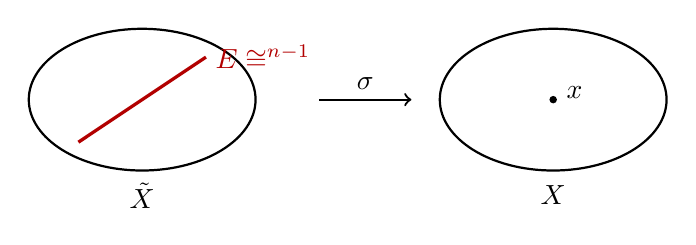
\begin{tikzpicture}[scale=0.9]
\draw[thick] (0,0) ellipse (1.6 and 1.0);\node at (0,-1.35) {$X$};\fill (0,0) circle (1.5pt);\node[right] at (0.05,0.1) {$x$};
\draw[->,thick] (-3.3,0)--(-2.0,0);\node[above] at (-2.65,0) {$\sigma$};
\begin{scope}[xshift=-5.8cm]
\draw[thick] (0,0) ellipse (1.6 and 1.0);\draw[very thick,red!70!black] (-0.9,-0.6)--(0.9,0.6);\node[red!70!black,right] at (0.9,0.6) {$E\cong\CP^{n-1}$};\node at (0,-1.35) {$\tilde X$};
\end{scope}
\end{tikzpicture}
\end{center}
\paragraph{(J) の証明。}完全列 $0\to\Oc(-2E)\to\Oc\to\Oc_{2E}\to0$ に $\sigma^*L^m$ をテンソルして
\[
H^0(\tilde X,\sigma^*L^m)\to H^0(2E,\sigma^*L^m|_{2E})\to H^1(\tilde X,\sigma^*L^m(-2E)).
\]
左は $H^0(X,L^m)$（$\sigma_*\Oc=\Oc$）、中央は $L^m\otimes\Oc_X/\mathfrak m_x^2$（次元 $n+1$。$0\to\Oc_E(-E)\to\Oc_{2E}\to\Oc_E\to0$ と $H^1(\CP^{n-1},\Oc(1))=0$ による）。したがって右端が $0$ なら (J)。$K_{\tilde X}$ の公式から
\[
\sigma^*L^m(-2E)=K_{\tilde X}\otimes B_m,\qquad B_m:=\sigma^*(L^m\otimes K_X^{-1})\otimes\Oc(-(n+1)E).
\]
\textbf{主張}：$m\gg0$ で $B_m$ は $\tilde X$ 上で正。すると Kodaira 消滅（定理 \ref{thm:kodaira}、$\tilde X$ に対して）から $H^1(\tilde X,K_{\tilde X}\otimes B_m)=0$ となり (J) が従う。
\emph{主張の理由}：$\Oc(-E)$ は $E$ に制限すると $\Oc_{\CP^{n-1}}(1)$ で正だが、$\tilde X$ 全体では $E$ に垂直な方向で正とは限らない。他方 $\sigma^*(i\Theta_{L})\ge0$ は、$E$ の接方向（$d\sigma$ の核）で $0$、他の方向で正である。計量を $E$ の近傍で適当にとり、2 つの形式 $A\ge0$（核 $=TE$）、$B$（$TE$ 上で正）に対し、コンパクト性から $mA+B$ は $m\gg0$ で正定値（核の方向では $B>0$、その外では $mA$ が支配）。$K_X^{-1}$ の項は有界で $m$ に吸収される。$E$ から離れた所では $\sigma$ が同型で $L^m$ の正値性が効く。
\paragraph{(S) の証明。}2 点 $x\ne y$ で爆発し $E_x,E_y$ をとる。$H^1(\tilde X,\sigma^*L^m(-E_x-E_y))=0$ を $K_{\tilde X}\otimes\big[\sigma^*(L^m\otimes K_X^{-1})(-n(E_x+E_y))\big]$ の正値性と Kodaira 消滅で示す。
\paragraph{一様性（$m_0$ が $x,y$ によらないこと）。}上の議論だけでは、$m$ の下限が $x,y$ に依存しうるように見える。$m_0$ を $x,y$ によらずに選べることは、\emph{コンパクト性}を使い、爆発上の正値性（$B_m$ が正になる $m$ の下限）の評価と消滅定理の適用が $x,y$ について一様にできることから従う（爆発の族について同じ議論をする）\tQ\ （ここでは骨子のみ。細部は文献）。\hfill$\square$

\begin{keybox}{要点（定理 \ref{thm:kodairaemb} の証明の構造）}
\textbf{仮定がどこで効くか}：(i) \emph{コンパクト}：$H^0$ が有限次元（射影空間への写像が定義される）、一様性、Kodaira 消滅。(ii) \emph{$L$ 正}：爆発上で $B_m$ が正（$m\gg0$）になり Kodaira 消滅が使える。(iii) 結論：消滅 $H^1=0\Rightarrow$ 切断が値と微分を与える（十分多くの切断）。統合論文が破れるとするのは (iii) の段（\S\ref{sec:unified}）。
\end{keybox}

\subsection{系：射影性の判定}
\begin{prop}[Lefschetz の $(1,1)$ 定理（コンパクト Kähler）]\label{prop:L11}\tP
$X$ をコンパクト Kähler、$\alpha\in H^2(X,\Z)$ とする。$\alpha$ の実係数像が $H^{1,1}(X)$ に入ることと、$\alpha=c_1(L)$ なる正則直線束 $L$ があることは同値。
\end{prop}
\begin{proof}
指数完全列 $\cdots\to H^1(\Oc^*)\xrightarrow{c_1}H^2(X,\Z)\to H^2(X,\Oc)$（第3巻）。右の写像は $\Z\to\Oc$ から来る。Dolbeault 同型 $H^2(X,\Oc)=H^{0,2}$ により、$\alpha$ の類の Hodge 分解での $(0,2)$ 成分への射影に等しい。よって $\ker=\{\alpha:\ \alpha^{0,2}=0\}$。実類なので $\alpha^{2,0}=\overline{\alpha^{0,2}}=0$ も同時に成り立ち、$\alpha\in H^{1,1}$ と同値。
\end{proof}
\begin{thm}[Kodaira の射影性判定]\label{thm:hodgemfd}\tP
コンパクト Kähler 多様体 $X$ で、Kähler 形式 $\omega$ の類 $[\omega]\in H^2(X,\mathbb R)$ が整類（$H^2(X,\Z)\to H^2(X,\mathbb R)$ の像の元。正の実数倍して整類にできればよい）なら、$X$ は射影的。
\end{thm}
\begin{proof}
$[\omega]$ が $H^2(X,\Z)$ の類 $\alpha$ の像とする。$\omega$ は閉 $(1,1)$ 形式なので $\alpha\in H^{1,1}$ で、命題 \ref{prop:L11} により $c_1(L)=\alpha$ の $L$ がある。$L$ に任意の計量 $h_0$ を入れると $\frac i{2\pi}\Theta_{h_0}$ も $c_1(L)$ を表す実閉 $(1,1)$ 形式で、$\omega-\frac i{2\pi}\Theta_{h_0}$ は完全な実閉 $(1,1)$ 形式。$\partial\bar\partial$-補題（定理 \ref{thm:ddbar}）で $\omega-\frac i{2\pi}\Theta_{h_0}=\frac i{2\pi}\partial\bar\partial\psi$（$\psi$ は実関数）。$h=e^{-\psi}h_0$ とおくと $\Theta_h=\Theta_{h_0}+\partial\bar\partial\psi$（$h=e^{-\varphi}$ なら $\Theta=\partial\bar\partial\varphi$）なので $\frac i{2\pi}\Theta_h=\omega>0$。$L$ は正で、Kodaira の定理により $X$ は射影的。
\end{proof}
（逆に射影的なら $\Oc(1)|_X$ が正で $[\omega_{FS}|_X]$ が整類。よって「射影的 $\iff$ 整類の Kähler 類をもつ」。）

\subsection{例}
\begin{ex}[$\CP^n$、Veronese 埋め込み]
$\Oc(m)$（$m\ge1$）は非常に豊富。$\varphi_{\Oc(m)}=\nu_m:\CP^n\to\CP^{\binom{n+m}m-1}$、$x\mapsto(x^a)_{|a|=m}$（Veronese）。$n=1$：有理正規曲線、$n=2,m=2$：Veronese 曲面 $\subset\CP^5$（問 \ref{p:veronese}）。
\end{ex}
\begin{ex}[曲線]
第4巻：$\deg L\ge2g+1$ なら $L$ は非常に豊富。(J) は $H^1(L(-2p))=0$、これは $\deg L(-2p)>2g-2$ ですでに Riemann--Roch が与える。Kodaira の方法（$K\otimes B$ の形に書く）でも同じ条件 $\deg L>2g$ が出る（問 \ref{p:curvejets}）。$n=1$ では爆発は不要。
\end{ex}
\begin{ex}[K3 曲面]
射影的な K3（例：4 次曲面）では $L$ の次数 $2g-2$ で $\CP^g$ に写る（例 \ref{ex:K3h0}）。一方、K3 曲面全体の 20 次元の変形族のうち、射影的なものは可算個の 19 次元の部分族（\S\ref{sec:ks}）。一般の K3 は Kähler だが射影的でない。
\end{ex}
\begin{ex}[$\CP^1\times\CP^1$ と Segre 埋め込み]\label{ex:segre}
$\Oc(a,b)$ は $a,b\ge1$ で非常に豊富。$h^0(\Oc(a,b))=(a+1)(b+1)$（Künneth）で、$\varphi_{\Oc(a,b)}=\mathrm{Segre}\circ(\nu_a\times\nu_b):\CP^1\times\CP^1\to\CP^{(a+1)(b+1)-1}$。$a=b=1$：$\CP^3$ の 2 次曲面 $z_0z_3=z_1z_2$（$[x_0y_0:x_0y_1:x_1y_0:x_1y_1]$）。$\Oc(1,0)$ は $\CP^1$ への射影を与えるだけで（豊富でない、境界）、$h^0=2$。ここまでの点で $K\otimes\Oc(a,b)$ の消滅の表（例 \ref{ex:P1P1}）が、豊富錐 $\{a,b>0\}$ の内部で消滅、境界と外側で破れることと対応している。
\end{ex}
\begin{ex}[曲線の埋め込み：次数 $2$ と $3$ の楕円曲線]
種数 $g=1$ の曲線 $X$ で $\deg L=d$ ならば $h^0(L)=d$（$d\ge1$）。$d=2$：$\varphi_L:X\to\CP^1$ は $2:1$ の被覆（埋め込みでない：$2g+1=3>2$）。$d=3$：$\varphi_L:X\to\CP^2$ は埋め込みで、像は平面 3 次曲線（$y^2=4x^3-g_2x-g_3$、$\wp$ 関数による）。これは (J) の条件 $\deg L>2g=2$ の最小の場合。$g=2$ では $\deg L\ge5$（$h^0=4$、$\CP^3$ への埋め込み）。第4巻の例とも一致。
\end{ex}
\begin{ex}[複素トーラスは射影的か]\label{ex:torusproj}
$T=\C^n/\Gamma$。$H^2(T,\Z)=\mathrm{Hom}(\Lambda^2\Gamma,\Z)$（交代整双線形形式 $E$）。$E\in H^{1,1}$ であることは $E(iu,iv)=E(u,v)$ と同値。$\omega_H$ が正 Kähler 形式のとき $E=\mathrm{Im}\,H$（$H$ は正定値 Hermite 形式）。定理 \ref{thm:hodgemfd} と逆から次を得る。
\begin{thm}[Riemann--Lefschetz]\tC\ （主張は Griffiths--Harris 第2章 \S6、Birkenhake--Lange）
$T=\C^n/\Gamma$ が射影的であることは、$\C^n$ 上の正定値 Hermite 形式 $H$ で $\mathrm{Im}\,H(\Gamma,\Gamma)\subset\Z$ をみたすもの（\emph{偏極}）が存在することと同値。
\end{thm}
$n=1$：$\Gamma=\Z+\Z\tau$ に対し $H(z,w)=z\bar w/\mathrm{Im}\,\tau$ とおくと $E=\mathrm{Im}\,H$ は $E(\tau,1)=1$ で $\Gamma$ 上整数値であり、\emph{楕円曲線は常に射影的}。$n\ge2$：$\Gamma=\Z[i]^n$ なら $H=\sum z_j\bar w_j$ で $\mathrm{Im}\,H(\Gamma,\Gamma)\subset\Z$、$T=E_i^n$ は射影的（問 \ref{p:torusPolar}）。一方、\emph{一般の} 2 次元トーラスは射影的でない：複素構造 $J$ が整な $J$-不変交代形式をもたないものがある。具体例を問 \ref{p:torusNS} で与える（$\Q(\sqrt2,\sqrt3)$ 上の厳密計算で $\NS=0$ を確かめた）。Hodge 数は同じ（例 \ref{ex:torusH}）なので、射影性は Hodge 数では見えない。
\end{ex}
\begin{ex}[Hopf 曲面]
Kähler でないので正の直線束も存在せず、射影的でない（問 \ref{p:hopfnopos}）。Kodaira の定理の逆の方向（射影的 $\Rightarrow$ Kähler）の対偶。
\end{ex}

\begin{keybox}{要点（\S\ref{sec:emb}）}
正 $\iff$ 豊富。証明は、爆発上の $K_{\tilde X}\otimes B_m$ に Kodaira 消滅 $\Rightarrow$ 切断が点と接ベクトルを分離。射影的 $\iff$ Kähler 類が整。複素トーラス：偏極（$\mathrm{Im}\,H$ が整）があるとき射影的。1 次元は常に射影的、一般の 2 次元以上は射影的でない。
\end{keybox}

\begin{prob}{基本}\label{p:veronese}
$\nu_2:\CP^2\to\CP^5$、$[x_0:x_1:x_2]\mapsto[x_0^2:x_0x_1:x_0x_2:x_1^2:x_1x_2:x_2^2]$ について、(a) 像が対称行列 $(y_{ij})$ の階数 $1$ の軌跡（$2\times2$ 小行列式 $=0$）に入ることを示せ。(b) $\nu_2$ が単射で immersion であることを確かめよ。(c) $h^0(\Oc(2))=6$ と整合することを確認せよ。
\end{prob}
\begin{prob}{標準}\label{p:curvejets}
種数 $g$ の曲線 $X$ と $\deg L>2g$ の直線束 $L$ について、任意の点 $p$ で $H^1(X,L(-2p))=0$ を、Serre 双対と Kodaira 消滅（1 次元、$\deg>0$ で $H^1(K\otimes\cdot)=0$）で示せ。これから $H^0(L)\to L\otimes\Oc/\mathfrak m_p^2$ が全射、すなわち $\varphi_L$ が $p$ で immersion かつ $p$ は基点でないことを導け。第4巻の $\deg\ge2g+1$ と比較せよ。
\end{prob}
\begin{prob}{標準}\label{p:torusPolar}
$\Gamma=\Z[i]^2\subset\C^2$、$H(z,w)=\sum z_j\bar w_j$ について、(a) $E=\mathrm{Im}\,H$ が $\Gamma$ 上整であることを示し、基底 $(1,0),(i,0),(0,1),(0,i)$ での行列と Pfaffian を求めよ。(b) $E$ は $E_i\times E_i$ の主偏極で、対応する $L=\mathrm{pr}_1^*\Oc(p_1)\otimes\mathrm{pr}_2^*\Oc(p_2)$（各因子 $E_i$ の点の因子）の $h^0$ が $|\mathrm{Pf}(E)|=1$ と一致することを（トーラス上の $h^0(L)=\chi(L)=\mathrm{Pf}$ を既知として）確かめよ。
\end{prob}
\begin{prob}{発展}\label{p:integralKahler}
(a) 定理 \ref{thm:hodgemfd} の証明を、符号に注意して再構成せよ（$h=e^{-\psi}h_0$ のとき $\Theta_h=\Theta_{h_0}+\partial\bar\partial\psi$）。(b) 結論として、「正の直線束 $L$ の曲率は、$c_1(L)$ の類に含まれる任意の Kähler 形式に取り替えられる」ことを示せ。(c) $\CP^n$ で $[\omega]=\frac12[\omega_{FS}]$ のとき、$[\omega]$ は整類か。この $\omega$ から得られる射影性の主張は何か。
\end{prob}
\begin{prob}{発展}\label{p:torusNS}
$\Z^4$ に実線形写像 $J$（$J^2=-1$）で複素構造を入れた 2 次元トーラス $T_J=(\mathbb R^4,J)/\Z^4$ について、$\NS(T_J)=\{E\in\Lambda^2(\Z^4)^*:\ E(Ju,Jv)=E(u,v)\}$。(a) $J_0$（標準）では $\mathrm{rank}\,\NS=4$（$T=E_i\times E_i$）。(b) $S=\begin{pmatrix}1&\sqrt2&\sqrt3&0\\0&1&0&0\\0&0&1&0\\\sqrt2&0&0&1\end{pmatrix}$、$J=SJ_0S^{-1}$ とする。$J^T E J=E$ を $E$ の 6 個の成分についての線形方程式とみて、$\Q(\sqrt2,\sqrt3)$ の基底 $1,\sqrt2,\sqrt3,\sqrt6$ で係数を分解し、有理解が $E=0$ のみであること（計算機で）を確かめよ。(c) 結論として $T_J$ に正の直線束はなく、射影的でないことを説明せよ。
\end{prob}

